\documentclass[11pt,a4paper]{article}
\usepackage[utf8]{inputenc}
\usepackage[T1]{fontenc}
\usepackage[spanish]{babel}
\usepackage[a4paper,top=4cm,bottom=2.5cm,left=2.5cm,right=2.5cm,headheight=3cm,headsep=.8cm]{geometry}
\usepackage{graphicx,amsmath,amssymb,booktabs,array,siunitx,multirow,float,caption,subcaption}
\usepackage[table]{xcolor}
\usepackage{fancyhdr,lastpage,enumitem,listings,microtype}
\microtypesetup{expansion=false}
\usepackage[colorlinks=true,linkcolor=blue!50!black,urlcolor=blue!50!black,citecolor=blue!50!black]{hyperref}
\graphicspath{{./imagenes/}}
\sisetup{output-decimal-marker={,},group-separator={.}}
\captionsetup{font=small,labelfont=bf}

\lstdefinestyle{python}{language=Python,basicstyle=\ttfamily\footnotesize,
 keywordstyle=\color{blue!70!black}\bfseries,commentstyle=\color{gray!70!black}\itshape,
 stringstyle=\color{red!60!black},showstringspaces=false,numbers=left,
 numberstyle=\tiny\color{gray},frame=single,rulecolor=\color{gray!40},breaklines=true,tabsize=4}
\lstset{style=python}

% Datos del informe (plantilla)
\newcommand{\TituloInforme}{Práctica No. 4:}
\newcommand{\NombrePractica}{Generación de variables aleatorias continuas}
\newcommand{\NombreUniversidad}{Universidad de los Llanos}
\newcommand{\NombreFacultad}{Facultad de Ciencias Básicas e Ingenierías}
\newcommand{\NombrePrograma}{Programa de Ingeniería de Sistemas}
\newcommand{\NombreCurso}{Simulación Computacional}
\newcommand{\TipoDocumento}{Informe de Laboratorio}
\newcommand{\FechaInforme}{Septiembre de 2026}
\newcommand{\Vacio}{}
\newcommand{\AlumnoUno}{J. Gregorio Delgado}
\newcommand{\CodUno}{160005010}
\newcommand{\AlumnoDos}{} \newcommand{\CodDos}{}
\newcommand{\AlumnoTres}{} \newcommand{\CodTres}{}
\newcommand{\AlumnoCuatro}{} \newcommand{\CodCuatro}{}

\newcommand{\LogoUniversidad}{%
 \IfFileExists{imagenes/logo_unillanos.png}
 {\includegraphics[height=2.7cm]{imagenes/logo_unillanos.png}}
 {\colorbox{gray!15}{\parbox[c][2.4cm][c]{3cm}{\centering\footnotesize Logo institucional}}}}
\pagestyle{fancy}\fancyhf{}\renewcommand{\headrulewidth}{0pt}
\fancyhead[L]{\parbox[c][2.8cm][c]{3.2cm}{\centering\LogoUniversidad}}
\fancyhead[C]{\parbox[c][2.8cm][c]{\dimexpr(\textwidth-4cm)/2\relax}{\centering\footnotesize
 \textbf{\MakeUppercase{\NombreUniversidad}}\\[2pt]Facultad de Ciencias Básicas e Ingenierías}}
\fancyhead[R]{\parbox[c][2.8cm][c]{\dimexpr(\textwidth-4cm)/2\relax}{\raggedleft\footnotesize
 Curso: \NombreCurso\\[2pt]\textbf{\TipoDocumento}}}
\fancyfoot[C]{\small Página \thepage\ de \pageref{LastPage}}

\begin{document}
\begin{center}
 {\LARGE\bfseries \TituloInforme}\\[6pt]
 {\normalsize\itshape \NombrePractica}\\[16pt]
 {\large \AlumnoUno\textsuperscript{1}}\\[12pt]
 {\small 1. Código: \CodUno, Ingeniería de Sistemas.}\\[10pt]
 {\small \NombreFacultad. \NombrePrograma.}\\[4pt]
 {\small Fecha: \FechaInforme}
\end{center}

\vspace{.4cm}\rule{\textwidth}{.6pt}
\begin{abstract}
Se implementaron métodos para generar variables aleatorias continuas y procesos de
conteo a partir de un generador congruencial mixto de período completo. Mediante
transformada inversa se obtuvieron cuatro muestras de 1000 observaciones y se
contrastaron sus histogramas con las densidades teóricas. También se simularon un
proceso de Poisson homogéneo, una variable Coxian y un proceso de Poisson no homogéneo
mediante adelgazamiento. Las medias y los conteos empíricos fueron cercanos a sus
valores teóricos, lo que respalda las implementaciones.

\medskip\noindent\textbf{Palabras clave ---} transformada inversa, Weibull,
generador congruencial, proceso de Poisson, Coxian, adelgazamiento.
\end{abstract}
\rule{\textwidth}{.6pt}

\section{Objetivos}
\begin{itemize}
 \item Generar variables aleatorias continuas a partir de uniformes pseudoaleatorios.
 \item Implementar y verificar el método de la transformada inversa.
 \item Generar variables Weibull y Coxian, y procesos de Poisson homogéneos y no homogéneos.
 \item Comparar resultados simulados con densidades, medias e intensidades teóricas.
\end{itemize}

\section{Consulta previa}
\begin{enumerate}[label=\arabic*.]
 \item \textbf{Variable aleatoria.} Es una función que asigna un número real a cada
 resultado de un experimento aleatorio y permite describir cuantitativamente su incertidumbre.
 \item \textbf{Distribución de probabilidad.} Es la regla que describe cómo se reparte
 la probabilidad entre los posibles valores de una variable; puede expresarse mediante
 una función de masa, una densidad o una función de distribución acumulada.
 \item \textbf{Distribución discreta frente a continua.} Una variable discreta toma un
 conjunto finito o numerable de valores y puede asignar probabilidad positiva a un punto.
 Una continua toma valores en intervalos, tiene probabilidad cero en cada punto aislado y
 sus probabilidades se obtienen integrando una densidad.
 \item \textbf{Distribución exponencial.} Para una tasa $\lambda>0$,
 \begin{equation}f(x)=\lambda e^{-\lambda x},\quad F(x)=1-e^{-\lambda x},\quad x\geq0.\end{equation}
 Su media es $1/\lambda$, su varianza $1/\lambda^2$ y posee falta de memoria.
 \item \textbf{Distribución Gamma.} Con forma $k>0$ y tasa $\lambda>0$,
 \begin{equation}f(x)=\frac{\lambda^k}{\Gamma(k)}x^{k-1}e^{-\lambda x},\quad x>0.\end{equation}
 Tiene media $k/\lambda$ y varianza $k/\lambda^2$. En la parametrización por escala,
 $\theta=1/\lambda$.
 \item \textbf{Normal estándar.} Es la normal con media $\mu=0$ y desviación estándar
 $\sigma=1$: $f(z)=(2\pi)^{-1/2}e^{-z^2/2}$, $z\in\mathbb{R}$.
 \item \textbf{Procesos de Poisson.} Ambos son procesos de conteo con incrementos
 independientes. En el homogéneo la tasa $\lambda$ es constante y los incrementos son
 estacionarios. En el no homogéneo la tasa depende del tiempo y el número medio de eventos
 en $(a,b]$ es $\int_a^b\lambda(t)\,dt$.
\end{enumerate}

\section{Fundamento teórico}
\subsection{Generador congruencial mixto}
La fuente uniforme utilizada fue
\begin{equation}X_{n+1}=(aX_n+c)\bmod m,\qquad U_n=\frac{X_n+0.5}{m},\label{eq:lcg}\end{equation}
con $m=2^{32}$, $a=1664525$ y $c=1013904223$. Por el teorema de Hull--Dobell,
el período es completo porque $c$ es coprimo con $m$, $a-1$ es divisible por el factor
primo 2 de $m$ y también por 4 \cite{ross2013}. El desplazamiento 0,5 evita exactamente 0 y 1.

\subsection{Transformada inversa}
Si $U\sim\mathcal{U}(0,1)$ y $F$ es continua e invertible, entonces $X=F^{-1}(U)$
tiene CDF $F$. Las inversas empleadas fueron:
\begin{align}
 X_a&=\ln(1+(e-1)U),\\
 X_b&=\begin{cases}2+2\sqrt{U},&U\leq1/4,\\6-\sqrt{12(1-U)},&U>1/4,\end{cases}\\
 X_c&=\frac{-1+\sqrt{1+8U}}{2},\\
 X_W&=\left(\frac{-\ln(1-U)}{\alpha}\right)^{1/\beta}.
\end{align}

\subsection{Poisson y Coxian}
Los tiempos entre eventos de un proceso de Poisson homogéneo son exponenciales:
\begin{equation}E_i=-\frac{\ln(U_i)}{\lambda},\qquad S_n=\sum_{i=1}^nE_i.\end{equation}
En una Coxian, la etapa $i$ dura un tiempo exponencial de tasa $\lambda_i$ y se
continúa con probabilidad $\alpha_i$. Su media es
\begin{equation}\operatorname{E}[X]=\sum_{i=1}^{k}\frac{\prod_{j=1}^{i-1}\alpha_j}{\lambda_i}.\label{eq:cox}\end{equation}
Para el proceso no homogéneo se usó adelgazamiento: se generan candidatos con una tasa
$M\geq\lambda(t)$ y se acepta el candidato en $t$ con probabilidad $\lambda(t)/M$.

\section{Equipos, materiales y herramientas}
\begin{table}[H]\centering
\caption{Recursos utilizados.}
\begin{tabular}{p{.27\textwidth}p{.6\textwidth}}\toprule
\textbf{Recurso}&\textbf{Descripción}\\\midrule
Equipo de cómputo&Computador personal.\\
Python&Implementación reproducible en un notebook Jupyter.\\
Bibliotecas&NumPy para cálculo vectorial y Pillow para las figuras.\\
Fuente&Capítulo 5 de Ross \cite{ross2013}.\\\bottomrule
\end{tabular}\end{table}

\section{Procedimiento o metodología}
\subsection{Validación del generador uniforme}
Se verificaron las condiciones de período completo y se generaron 1000 uniformes con
semilla 160005010. Se obtuvo media 0,5100 y varianza 0,0844, cercanas a 0,5 y
$1/12=0,0833$.

\subsection{Variables aleatorias continuas}
Se generaron 1000 observaciones por inciso con semillas distintas. Para Weibull, la guía
no fija parámetros; se seleccionaron $\alpha=1,5$ y $\beta=2$, editables en el notebook.
Cada muestra se resumió mediante su media y un histograma normalizado superpuesto a la
densidad teórica. Para el inciso b se integró por tramos:
\begin{equation}F_b(x)=\begin{cases}(x-2)^2/4,&2\leq x\leq3,\\x-x^2/12-2,&3<x\leq6.\end{cases}\end{equation}

\subsection{Poisson homogéneo y Coxian}
Se escogieron $T=10$ y $\lambda=2$ y se acumularon tiempos exponenciales hasta superar
$T$. Para la Coxian se usaron cuatro etapas:
\begin{equation}(\lambda_1,\ldots,\lambda_4)=(1,0;1,4;0,9;1,8),\quad
(\alpha_1,\alpha_2,\alpha_3)=(0,85;0,70;0,55).\end{equation}
Se simularon 1000 valores para contrastar la media con la Ecuación~\eqref{eq:cox}.

\subsection{Poisson no homogéneo}
La intensidad de la guía fue
\begin{equation}\lambda(t)=\begin{cases}t/5,&0<t<5,\\1+5(t-5),&5\leq t<10.\end{cases}\end{equation}
Su máximo es 26, usado como tasa candidata. La intensidad integrada es
\begin{equation}\Lambda(10)=\int_0^5\frac{t}{5}\,dt+\int_5^{10}[1+5(t-5)]\,dt=70,\end{equation}
por lo que se esperan 70 eventos en promedio.

\section{Resultados y análisis}
\subsection{Distribuciones continuas}
\begin{table}[H]\centering
\caption{Comparación de medias para 1000 observaciones.}\label{tab:medias}
\begin{tabular}{lrrr}\toprule
\textbf{Distribución}&\textbf{Empírica}&\textbf{Teórica}&\textbf{Error}\\\midrule
Inciso a&0,5769&0,5820&-0,0051\\
Inciso b&3,6627&3,6667&-0,0040\\
Inciso c&0,5749&0,5833&-0,0084\\
Weibull $(\alpha=1,5,\beta=2)$&0,7274&0,7236&+0,0038\\\bottomrule
\end{tabular}\end{table}

\begin{figure}[H]\centering
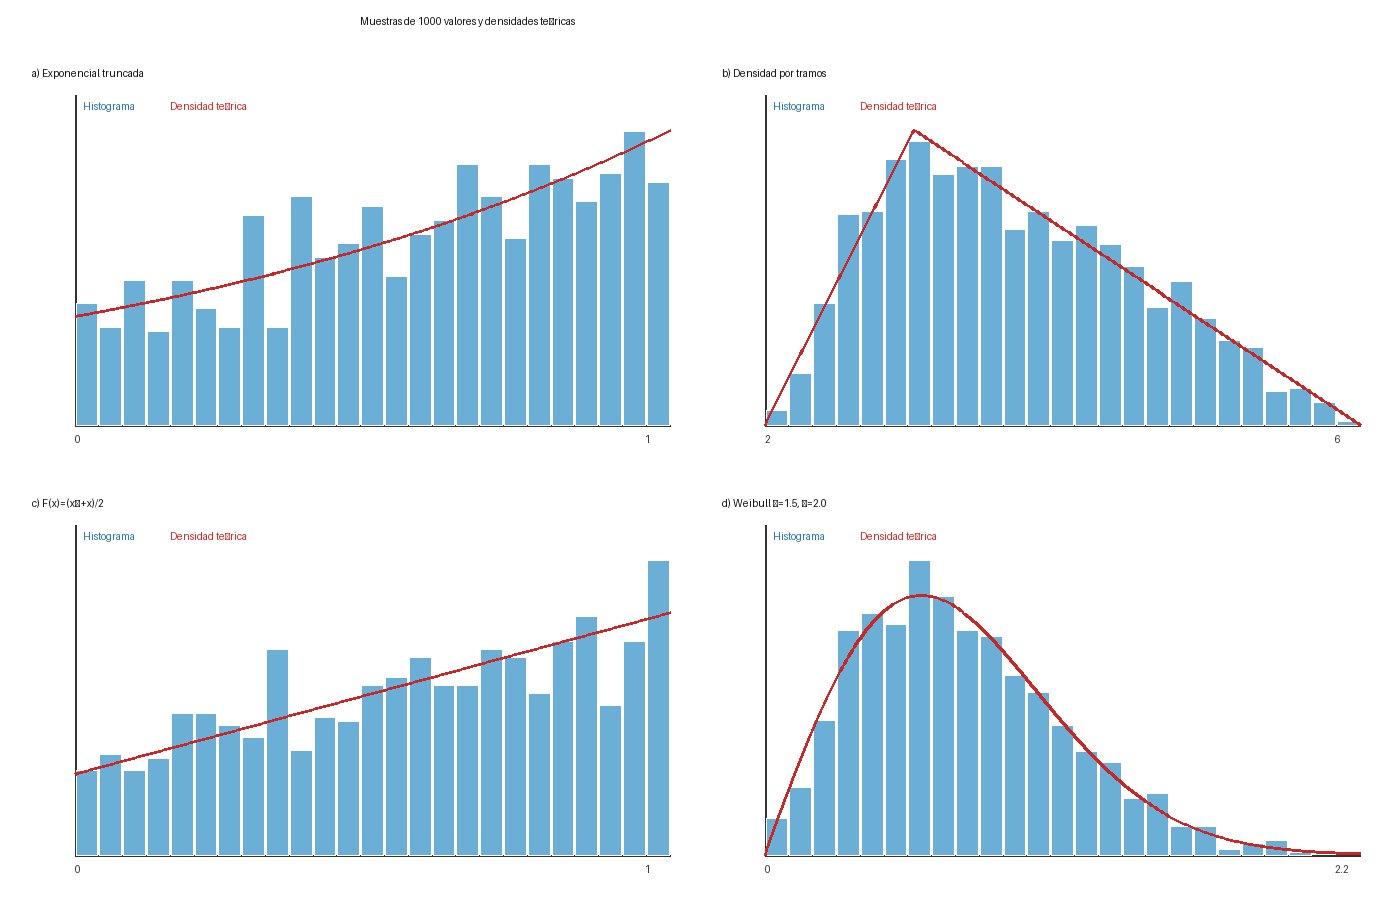
\includegraphics[width=\textwidth]{distribuciones_continuas.png}
\caption{Histogramas normalizados y densidades teóricas.}\label{fig:dist}
\end{figure}
Los histogramas reproducen las formas esperadas: crecimiento exponencial en a, cambio
de pendiente en b, crecimiento lineal en c y forma unimodal en Weibull. Los errores
absolutos de las medias fueron inferiores a 0,009; las diferencias restantes son
variación de Monte Carlo.

\subsection{Poisson homogéneo y Coxian}
El proceso homogéneo produjo 18 eventos en $[0,10]$, frente a
$\operatorname{E}[N(10)]=20$. Los tiempos fueron 0,420; 1,659; 1,916; 2,426; 2,451;
3,218; 5,243; 5,850; 6,297; 6,558; 6,595; 6,878; 6,915; 7,211; 7,794; 7,851;
9,343 y 9,349.

La media Coxian empírica fue 2,4186 y la teórica 2,4501. De las 1000 trayectorias,
151 terminaron en la etapa 1, 274 en la 2, 260 en la 3 y 315 alcanzaron la 4. La
cercanía entre medias valida la generación exponencial y las decisiones de continuación.

\subsection{Poisson no homogéneo}
Se generaron 264 candidatos y se aceptaron 68, cerca de $\Lambda(10)=70$. Los primeros
tiempos aceptados fueron 2,247; 4,276; 4,718; 5,280; 6,005; 6,222; 6,407; 6,459;
6,665; 6,803; 6,860; 7,044; 7,080; 7,121 y 7,196.

\begin{figure}[H]\centering
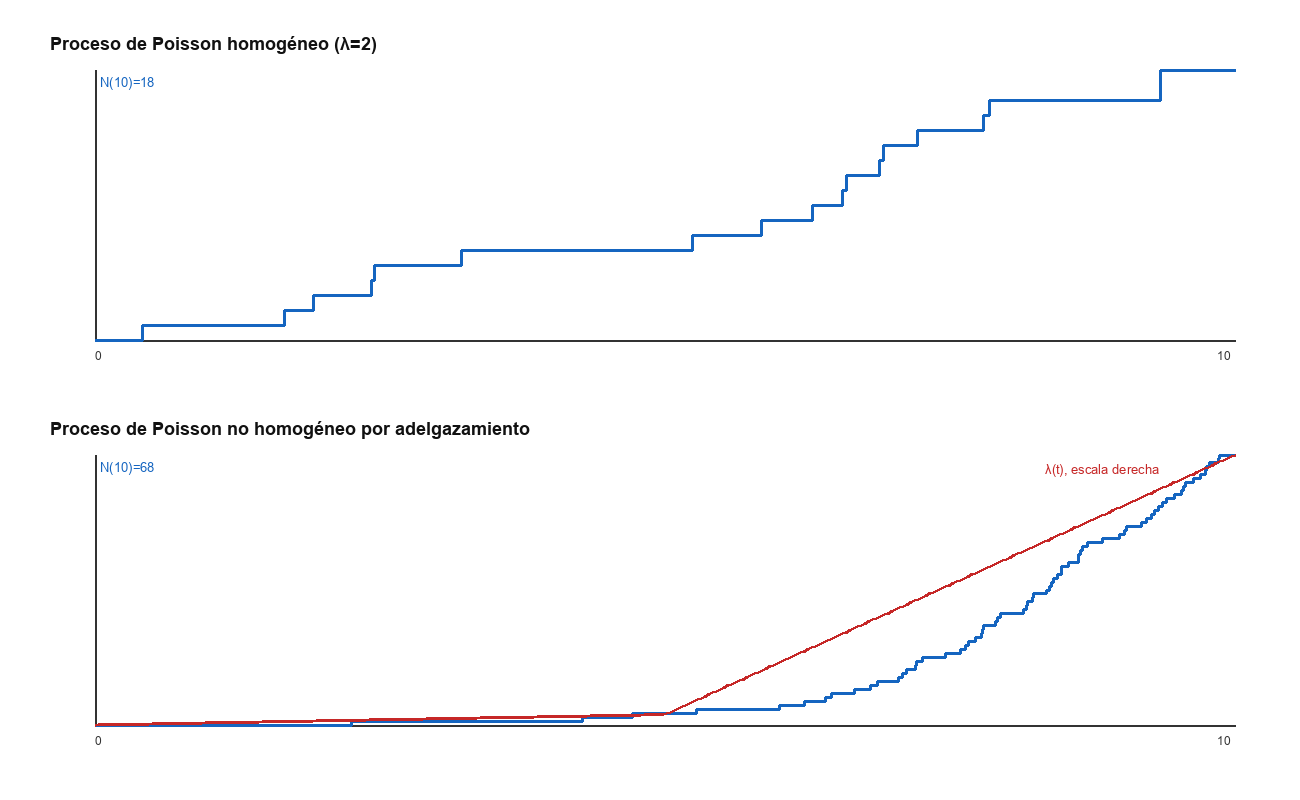
\includegraphics[width=\textwidth]{procesos_poisson.png}
\caption{Trayectorias homogénea y no homogénea; en rojo, la forma de $\lambda(t)$.}\label{fig:poisson}
\end{figure}
En la trayectoria homogénea la pendiente media del conteo es aproximadamente constante.
En la no homogénea hay pocos eventos al inicio y una concentración fuerte después de
$t=5$, coherente con el aumento de la intensidad. Que los totales no sean exactamente
20 y 70 es esperado: esos valores son medias, no resultados deterministas.

\section{Conclusiones}
\begin{itemize}
 \item La transformada inversa produjo las cuatro variables solicitadas y la comparación
 de medias e histogramas respaldó la corrección de las muestras.
 \item El generador congruencial cumple las condiciones de período completo y produjo
 estadísticas uniformes cercanas a las teóricas.
 \item La acumulación de exponenciales reproduce Poisson; la Coxian incorpora decisiones
 probabilísticas de permanencia entre etapas.
 \item El adelgazamiento reprodujo la intensidad no constante: los eventos se concentraron
 donde $\lambda(t)$ aumentó.
 \item Las semillas fijas hacen totalmente reproducibles los resultados presentados.
\end{itemize}

\begin{thebibliography}{9}
\bibitem{ross2013} S. M. Ross, \textit{Simulation}, 5th ed. Pearson, 2013, cap. 5.
\end{thebibliography}
\end{document}
